\documentclass[border=10pt]{standalone}
\usepackage{pgfplots}
\pgfplotsset{compat=1.17}
\begin{document}
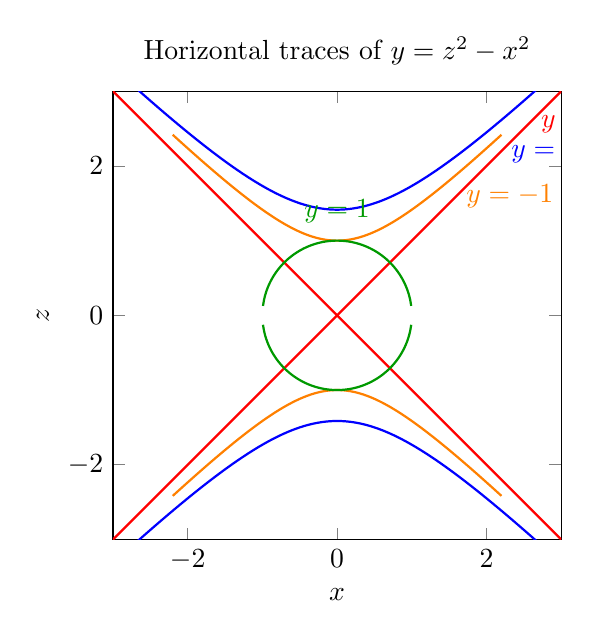
\begin{tikzpicture}
\begin{axis}[
    xlabel=$x$,
    ylabel=$z$,
    title={Horizontal traces of $y=z^2-x^2$},
    axis equal image,
    xmin=-3, xmax=3,
    ymin=-3, ymax=3,
]
\addplot[blue, thick, domain=-2.8:2.8, samples=200] {sqrt(x^2+2)};
\addplot[blue, thick, domain=-2.8:2.8, samples=200] {-sqrt(x^2+2)};
\addplot[orange, thick, domain=-2.2:2.2, samples=200] {sqrt(x^2+1)};
\addplot[orange, thick, domain=-2.2:2.2, samples=200] {-sqrt(x^2+1)};
\addplot[red, thick, domain=-3:3, samples=200] {x};
\addplot[red, thick, domain=-3:3, samples=200] {-x};
\addplot[green!60!black, thick, domain=-1.4:1.4, samples=200] {sqrt(1-x^2)};
\addplot[green!60!black, thick, domain=-1.4:1.4, samples=200] {-sqrt(1-x^2)};
\node[blue, anchor=west] at (axis cs:2.2,2.2) {$y=-2$};
\node[orange, anchor=west] at (axis cs:1.6,1.6) {$y=-1$};
\node[red, anchor=west] at (axis cs:2.6,2.6) {$y=0$};
\node[green!60!black, anchor=south] at (axis cs:0,1.1) {$y=1$};
\end{axis}
\end{tikzpicture}
\end{document}
